\documentclass[10pt,twocolumn,letterpaper]{article}
\usepackage[english]{babel}
\usepackage{graphicx}
\usepackage{times}
\usepackage{epsfig}
\usepackage{graphicx}
\usepackage{amsmath}
\usepackage{amssymb}
\usepackage{array}
\usepackage{float}
\usepackage[english]{babel}
\setcounter{page}{1}
\usepackage{dblfloatfix}    % To enable figures at the bottom of page
\begin{document}

%%%%%%%%% TITLE
\title{CRISPEY- ML}

\author{Shi-An  A. Chen and Elizabeth Tran \\
Stanford University\\
{\tt\small { shian, eliztran @ stanford.edu}}\\
}
\maketitle

%%%%%%%%% ABSTRACT
\begin{abstract}
Direct precision genome editing allows for the understanding of genetic blueprint that directs activities of a living organism. CRISPR-Cas9 is a system that provides scalable means to perform precise genome editing, followed by functional readouts of cellular-and organism-level phenotypes. To ensure accuracy in the phenotypic readout, prediction of off-target effects of CRISPR-Cas9 has been the main focus in the field of genome editing technology development.
With the increasing availability of high-quality functional data specifically designed for off-target evaluation, there have been tremendous strides in constructing models for predicting off-target. Here, we analyze the off-target effects of several hyperparameters on the off-target effects of CRISPEY, a novel gene editing approach based on CRISPR-Cas9, using several machine learning algorithms. Using support vector machines (SVMs), we were able to classify editing elements that are prone to off-targeting at 60 \%\ recall rate. This model will greatly improve our ability to exclude off-target edits from precision editing studies, thus reducing experimental noise and reagent cost.
\end{abstract}
%%%%%%%%% BODY TEXT


%%%%%%%%% Intro
\section*{Introduction}
Genetic variation is the key to successful adaptive evolution: genotype changes can lead to changes in phenotype and thus individual fitness. The majority of these variants are unlikely to impact human phenotype or health, but there is a number that has been connected to diseases and more yet to be discovered. Being able to shed light onto the functional consequence of rare variants as well as the genetic differences will give insight to which variants are selectively advantageous to disease, development, and survival. However, identifying the genetic variants to implement such a strategy has been an ongoing challenge.

CRISPR (clustered regularly interspaced short palindromic repeats)-Cas9 is a gene editing technique that introduces precise changes to the genome by programming molecules called guide RNAs. The Cas9 protein will then carry the guide RNA to the target genomic region, where guide RNA and target DNA completely matches, followed by the introduction of a double-stranded break in the DNA. The break can be repaired by incorporating externally supplied of DNA templates that carry an alternative variant of the DNA. This repair process will result in the replacement of the original variant with the alternative variant, and the edited cell or organism can be assayed for phenotype. If a change in the relevant phenotype is observed, we can assume the alternative variant is causal for the phenotypic change, since the rest of the genome remain unchanged. The programmable nature of CRISPR-Cas9 and its ease of use has been a popular tool to study the effects of genetic variants in model organisms and human cells. More excitingly, once the disease causing variant is determined, it is possible to therapeutically deliver CRISPR-Cas9 into patient tissues to replace the disease variant with a non-disease variant, thus curing the disease.

Off-targeting is a phenomenon where the Cas9 protein introduces double-stranded breaks to a DNA that the guide RNA does not completely match with, resulting in non-intentional changes elsewhere in the genome. In a research setting, off-target effects will introduce experimental noise and hinder our ability to locate the causal variant. In a therapeutic standpoint, off-targeting of CRISPR-Cas9 will introduce unwanted mutations to the patient, leading to unknown health risks. To prevent choosing guide RNAs that are prone to have off-target effects, we would need to gain knowledge on the specific features on these guide RNAs. Machine learning, in this case, can play a role in classifying off-target prone guide RNAs, allowing us to select the best guide RNAs to be used in research and therapeutics. In addition, by extracting the feature that are predictive of guide RNA off-target activities will help us learn about the sequence to function relationship of guide RNAs that CRISPR-Cas9 activity is dependent on. Lastly, the obtained model will be useful for setting up a framework for evaluating other genome editing tools that use sequence-dependent, programmable DNA nucleases other than Cas9.
\section*{Background}
CRISPEY (Cas9 retron precise parallel editing via homology), a novel genome-editing technique developed at Stanford in 2018, empirically measures in parallel the fitness effects of thousands of natural genetic variants in yeast at single-base resolution. This editing approach was able to discover hundreds of variants affecting fitness, giving us enough statistical power to show that these variants are enriched for genomic features such as promoters and transcription factor (TF) binding sites. Unexpectedly, the study also generated data on off-target effects for the thousands of guide RNAs that are used for variant editing, empirically measured by cellular toxicity during editing. This data set is a rich resource for modeling off-target effect with thousands of guide RNAs, compared to previous studies that typically only look at most a few dozen guide RNAs. Here, we explore a variety of machine learning techniques to model the CRISPEY dataset, with the goal to predict reliable guide RNAs that are less prone to off-targeting. Specifically, we use the CRISPEY dataset from Sharon et al to extract guide RNA features as input and off-target effect as labels.
With the advent of deep neural networks (DNN), there have been groundbreaking improvements in feature representation (Krizhevsky et al., 2012), object classification, to pattern recognition (He et al., 2016). DNNs utilize stacked layers of nonlinear operations instead of manually extracting features from input data and its multi-layers learning can get a more effective expression. However, there have not been many deep learning applications for CRISPR-Cas9 off-target prediction (Chuai et al., 2018; Lin \&\ Wong, 2018). 
\begin{table}[]
	\begin{tabular}{llr}
		\hline
		\multicolumn{3}{c}{Model Performance}    \\ \cline{1-3}
		Model Type & SVM   & Logistic Regression \\ \hline
		Accuracy   & 38.78 &         94            \\
		Precision  & 1.18  &          2.20           \\
		Recall     & 59.64 &                 8.77    \\
	\end{tabular}
	\caption{\label{tab: Model Scores}Model Scores}
\end{table}

%%%%%%%%% Methods
\section*{Methods}
There have been several scoring methods that have been used to analyze this form of data target prediction methods, e.g., cumulative distribution function (CDF), MIT, CROPIT , CCTOP, and traditional machine learning models. As a baseline performance,  we will be using these methods to assess our model's accuracy. 
\section*{Preprocessing}
DNA analysis requires first converting DNA sequences (20 basepairs in {A,T,C,G}) to numbers and one hot encoding is a way to represent categorical data as binary vectors. Similarly to preprocessing from Lin \&\ Wong, we adapted Python's SciKit Learn library to works with the DNA sequences. Refer to Figure 1 to see an example of what one hot coding for a DNA sequence could be. Our total amount of data with preprocessing, after removing sequences that were labeled with no effect, was a total of 23,936 samples. However, the classes were imbalanced (249 samples in effect and 18,468 in no-effect). 

Due to the imbalance of our classes, we implemented SMOTE (Synthetic Minority Oversampling Technique) algorithm from Python’s Imblearn Library that creates synthetic observations of the minority class by 1). Finding the k-nearest-neighbors for minority class observations and 2). Randomly choosing one of the k-nearest neighbors to use it to create a similar but random tweaked, new observation. We chose to upsample to a class ratio of 2.0. Our dataset consisted of a total of 36,856 training samples (18,468 for effect and no effect samples respectively and 4,670 testing samples. This will then allow us to identify relevant features for predicting variant fitness. 
\section*{Results}
In order to better understand the dataset, we first approached our analysis using several traditional machine learning techniques. 

\textit{Logistic Regression \\}
As an initial step, we ran a logistic regression model due to our data being binary dataset. Even though our accuracy score does a bit better than random guessing, changing the hyperparameters does not help increase performance.  Our highest performing accuracy is  94$\%$; however, because there is a class imbalance, although using SMOTE addresses some of the issues, the score we are hoping to be high is our recall score. The recall score here is 8.77$\%$. Refer to Table 1 to details on our performance. 

\textit{Support Vector Machine\\}
Following, our next approach we ran a support vector machine (SVM) model. Our SVM performance for accuracy is low (38.78 $\%$), however, the recall score, here, is better than random guessing being 59.64$\%$. Refer to Figure 1 for our ROC curve  and Table 1 for details on our overall performance. 

\section*{Discussion}
As an initial step of constructing traditional machine learning method models, we were able to better understand our data. Following this, we are planning to apply another two other types of algorithms to analyze our dataset. One of them being random decision forests and the other being neural networks. We want to use a random decision forest, because this method is highly data adaptive, applies to large a p and small n problems, and is able to account for correlation as well as interactions among features. For our neural network, we are planning to use the Lin \&\ Wong model structure as our baseline network architecture. We are choosing to use their model as a baseline structure because the dataset that they conducted the model upon is similar to how Sharon et al. curated their dataset. Refer to Table 2 for an outline of their model’s structure.  However, the difference between Lin \&\ Wong and Sharon et al. datasets is that instead of having one dataset to construct their model, they chose to combine multiple datasets (CRISPOR dataset (Tsai et al., 2015) and GUIDE-seq dataset (Jean-Paul \&\ Haeussler, M. 2018) which still has fewer positive labels (143 and 28 positive respectively) than Sharon et al (249 positive). We believe that if  Lin \&\ Wong dataset was able to perform with such high accuracy, we will be able to have a similar performance as well because the Sharon et al dataset has a more diverse set of guide RNA sequence. 

\begin{figure}
	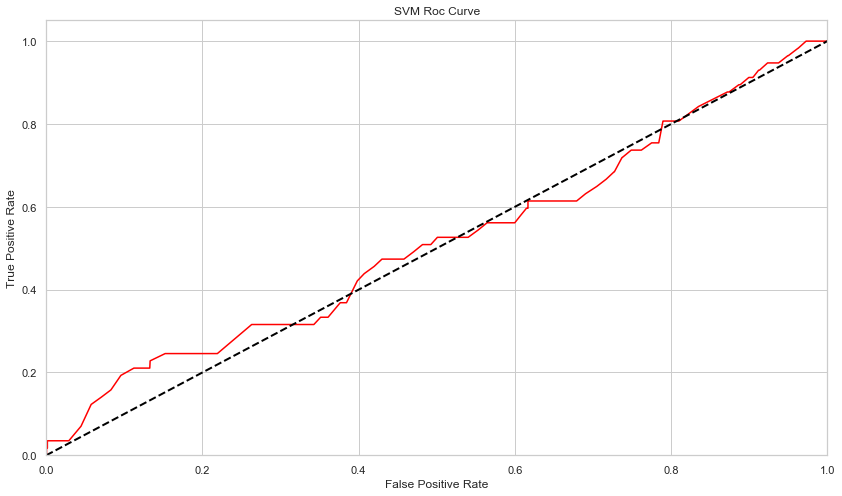
\includegraphics[width=\linewidth,height=\textheight,keepaspectratio]{SVM_I}
	\caption{SVM ROC Curve }
\end{figure}
	
	
\section*{References}	

Chawla, N. V., Bowyer, K. W., Hall, L. O., \&\ Kegelmeyer, W. P. (2002). SMOTE: synthetic minority over-sampling technique. Journal of artificial intelligence research, 16, 321-357.

Chuai, G., Ma, H., Yan, J., Chen, M., Hong, N., Xue, D., Zhou, C., Zhu, C., Chen, K., Duan, B., et al.(2018). DeepCRISPR: optimized CRISPR guide RNA design by deep learning. Genome Biol. 19, 80.

He, K., Zhang, X., Ren, S., \&\ Sun, J. (2016). Deep residual learning for image recognition. In Proceedings of the IEEE conference on computer vision and pattern recognition (pp. 770-778).

Jean-Paul, C. \&\ Haeussler, M. (2018). CRISPOR: intuitive guide selection for CRISPR/Cas9 genome editing experiments and screens. Nucleic Acids Res. 46, W242–W245.

Krizhevsky, A., Sutskever, I., \&\ Hinton, G. E. (2012). Imagenet classification with deep convolutional neural networks. In Advances in neural information processing systems (pp. 1097-1105).

Lin, J., Wong, K.-C. (2018). Off-target predictions in CRISPR-Cas9 gene editing using deep learning. Bioinformatics. 34, i656–i663.

Sharon, E., Chen, S. A. A., Khosla, N. M., Smith, J. D., Pritchard, J. K., \&\ Fraser, H. B. (2018). Functional genetic variants revealed by massively parallel precise genome editing. Cell, 175(2), 544-557

Tsai, S.Q., Zheng, Z., Nguyen, N.T., Liebers, M., Topkar, V.V., Thapar, V., Wyvekens, N., Khayter, C., Iafrate, A.J., Le, L.P., et al. (2015). GUIDE-seq enables genome-wide profiling of off-target cleavage by CRISPR-Cas nucleases. Nat. Biotech. 33, 187–197.

\begin{table}[]
	\begin{tabular}{|l|l|}
		\hline
		\textbf{Baseline Model}                   \\ \hline
		Convo Layer- filter 40, kernal size: 4 × 1               \\ \hline
		Batch Normalization                                    \\ \hline
		Max-Pooling - filter 1x5, stride 5                     \\ \hline
		Convo Layer- filter 40, kernal size: 4 × 2                 \\ \hline
		Batch Normalization                                       \\ \hline
		Max-Pooling - filter 1x5, stride 5                    \\ \hline
		Convo Layer- filter 40, kernal size: 4 × 2                 \\ \hline
		Batch Normalization                                       \\ \hline
		Max-Pooling - filter 1x5, stride 5                        \\ \hline
		Convo Layer- filter 40, kernal size: 4 × 3                 \\ \hline
		Batch Normalization                                        \\ \hline
		Max-Pooling - filter 1x5, stride 5                      \\ \hline
		Convo Layer- filter 40, kernal size: 4 × 5                \\ \hline
		Batch Normalization                                         \\ \hline
		Max-Pooling - filter 1x5, stride 5                          \\ \hline
		Flatten - 200                                              \\ \hline
		ReLu                                                    \\ \hline
		Fully-Connected 100                                       \\ \hline
		Fully-Connected 23                                        \\ \hline
		Dropout -  .15                                          \\ \hline
		Softmax - 2                                       \\ \hline
		
	\end{tabular}
	\caption{\label{tab: Model Arch} Neural Network Structure}
\end{table}
%-------------------------------------------------------------------------


\end{document}
